\section{Construction (5 points)}

\begin{center}
	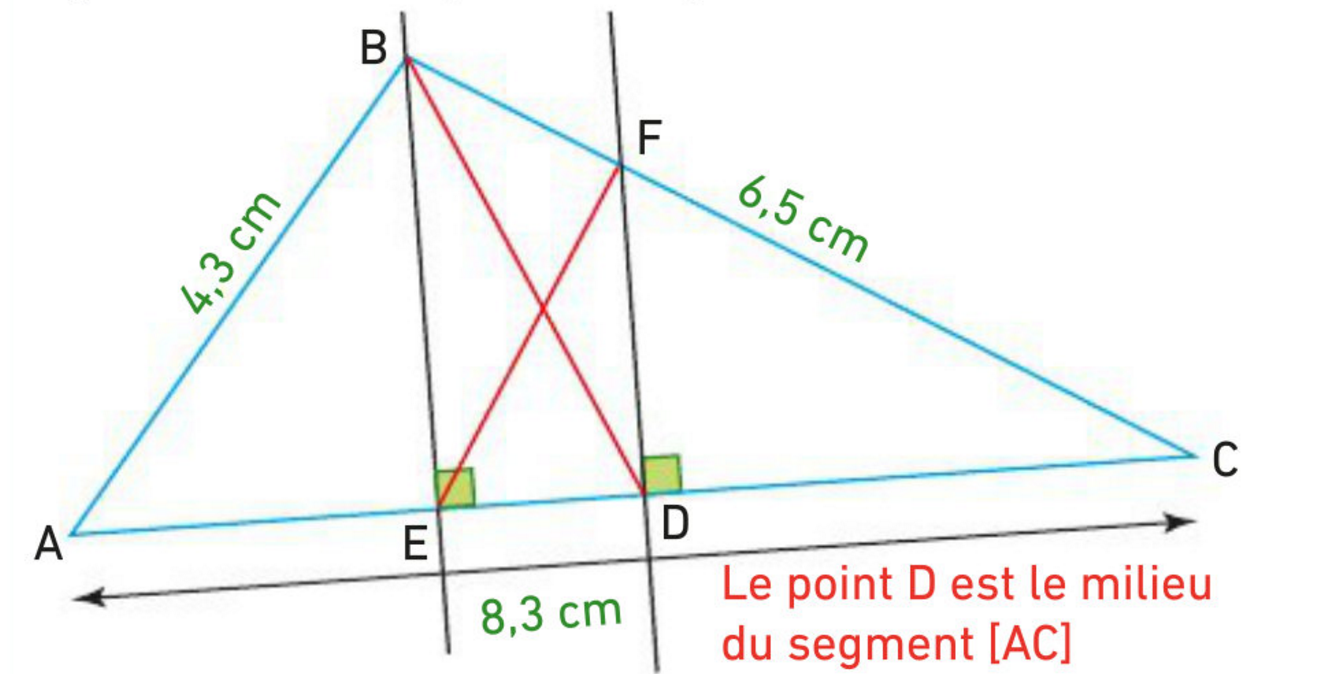
\includegraphics[scale=0.3]{img/triangle}
\end{center}

\begin{questions}
	
	\question[1\half] Comment décrire la droite $(BE)$ ?
	\begin{solution}
		$(BE)$ est la hauteur issue de B.
	\end{solution}
	
	\question[1\half] Comment décrire la droite $(DF)$ ?
	\begin{solution}
		$(DF)$ est la médiatrice de $[AC]$.
	\end{solution}
	
	\question[2] Rédiger un programme de construction de cette figure.
	\begin{solution}
		\begin{itemize}
			\item Construire un triangle $ABC$, tel que $AB$=\num{4.3} cm, $BC$ = \num{6.5} cm et $AC$=\num{8.3} cm.
			
			\item Tracer la hauteur issue de $B$, son pied est le point $E$. Coder la figure.
			
			\item Tracer la médiatrice de $[AC]$, elle coupe $(AC)$ en $D$ et $(BC)$ en F. Coder la figure
			
			\item Tracer les segments $[BD]$ et $[EF]$. 
		\end{itemize}
	\end{solution}
	
	
\end{questions}
  